\section{Method}
\label{sec:method}

We introduce GraphIV (Graph + arXiv), an open citation intent graph of arXiv, alongside BoundedField, a tunable, LLM-free, citation-aware retriever, and GraphIV-MCP, a suite of research tools. To keep GraphIV self-hostable, everything was built and tested on one consumer machine: an AMD Ryzen 7 7700X, 64 GB of memory, and an NVIDIA RTX 3090.

\subsection{Dataset}
\label{sec:dataset}

\begin{figure*}[t]
\centering
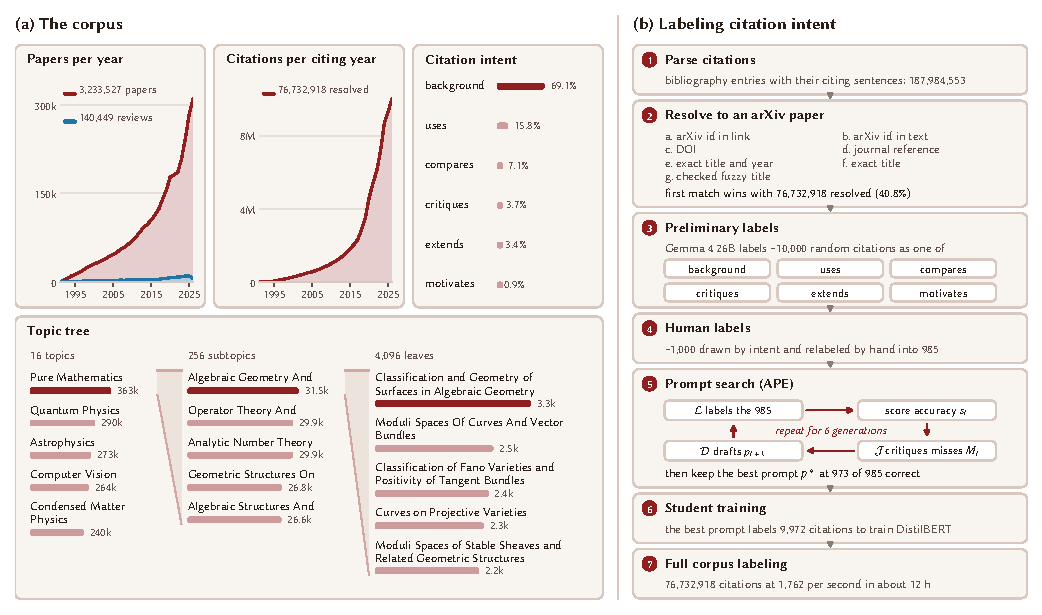
\includegraphics[width=\textwidth]{figures/dataset.pdf}
\Description{Two panels. Panel (a), the corpus, has four charts. Papers per year rises from near zero in the early 1990s to about 300 thousand a year by 2025, for 3,233,527 papers, with reviews a thin line below it totaling 140,449. Resolved citations per citing year rise steeply after 2015 to 76,732,918 in all. Citation intent is a bar chart: background 69.1\%, uses 15.8\%, compares 7.1\%, critiques 3.7\%, extends 3.4\%, motivates 0.9\%. The topic tree shows 16 topics, led by Pure Mathematics with 363 thousand papers, then Quantum Physics, Astrophysics, Computer Vision, and Condensed Matter Physics; 256 subtopics, led by Algebraic Geometry with 31.5 thousand; and 4,096 leaves, led by classification and geometry of surfaces in algebraic geometry with 3.3 thousand. Panel (b), labeling citation intent, is a seven-step pipeline from top to bottom: parse 187,984,553 citations with their citing sentences; resolve each to an arXiv paper by seven strategies in order, the first match winning, resolving 76,732,918 (40.8\%); Gemma 4 26B labels about 10,000 random citations as one of six intents; about 1,000 drawn by intent are relabeled by hand into 985; a prompt search loop in which the labeler labels the 985, the accuracy is scored, the judge critiques the misses, and the drafter writes the next prompt, repeated for six generations, keeping the best prompt at 973 of 985 correct; the best prompt labels 9,972 citations to train a DistilBERT student; and the student labels all 76,732,918 citations at 1,762 per second in about 12 hours.}
\caption{GraphIV's overview. (a) The corpus as broken down per year alongside its citation intent and topic tree. (b) The citation intent labeling pipeline, in which the labeler $\mathcal{L}$, judge $\mathcal{J}$, and drafter $\mathcal{D}$ search for the teacher prompt.}
\label{fig:dataset}
\end{figure*}

GraphIV was built from Cornell's arXiv metadata snapshot on Kaggle \citep{clement2019arxiv}, which is free and updated biweekly. Each alternative misses one of these: Semantic Scholar's bulk datasets require an API key\footnote{\furl{https://semanticscholar.org/product/api}} \citep{kinney2023s2}, OpenAlex's free snapshot is quarterly and its daily one paid\footnote{\furl{https://help.openalex.org/access/pricing}} \citep{priem2022openalex}, and unarXive, the closest predecessor, is frozen at 2022 \citep{saier2023unarxive}. As the snapshot holds only per-paper metadata, we built the citation graph from arXiv's open HTML renders. As of 2026-11-11, the corpus held 3,233,527 papers, 3,196,302 of them processed.

\paragraph{Citation extraction and resolution:}
For each paper with an HTML version, we parsed its bibliography and the sentences citing each entry. As arXiv bibliographies follow no single convention, we resolved citations with the strategies in \cref{tab:resolution}. Of 187,984,553 parsed citations, 76,732,918 (40.8\%) resolved to a paper in the corpus.

\begin{table}[t]
\caption{Citation resolution strategies. Numbers shown correspond to additional citations resolved after a method is employed.}
\label{tab:resolution}
\centering
\small
\begin{tabular}{lr}
\toprule
Method & Citations \\
\midrule
arXiv id in the text & 21,831,361 \\
Exact title and year & 16,478,534 \\
Journal reference & 13,397,614 \\
arXiv id in the link & 10,058,637 \\
Fuzzy title & 8,491,441 \\
DOI & 4,108,520 \\
Exact title, year disagrees & 2,366,811 \\
\midrule
Resolved & 76,732,918 \\
Fuzzy match rejected & 18,253,288 \\
No match & 92,998,347 \\
\midrule
Parsed & 187,984,553 \\
\bottomrule
\end{tabular}
\end{table}

\paragraph{Citation intent:}
We classified each citation into one of six intents: \term{background}, \term{uses}, \term{compares}, \term{extends}, \term{critiques}, and \term{motivates}. Existing classifiers are coarser: SciCite uses background, method, and result comparison \citep{cohan2019scaffolds}, while ACL-ARC and MultiCite separate extending from comparing but fold critiques into comparison \citep{jurgens2018citation,lauscher2022multicite}. We kept \term{critiques} separate since, with \term{extends} and \term{compares}, it forms what our lineage tracing follows.

As labeling 76.7 million citations with an LLM on one GPU is not computationally realistic, we distilled one into a small classifier (\cref{fig:dataset}b). Gemma 4 26B \citep{gemmateam2026gemma4} labeled 10,000 random citations, from which a stratified sample of about 1,000 was relabeled by hand, leaving 985 human-labeled citations $\{(x_i, y_i)\}_{i=1}^{n}$. Against these, we ran automatic prompt engineering \citep{zhou2023ape}: at generation $t$, the labeler $\mathcal{L}$ labeled every citation under prompt $p_t$, the judge $\mathcal{J}$ critiqued $p_t$ from its misses alone, and the drafter $\mathcal{D}$ wrote the next prompt from the critique (\cref{eq:ape}).
\begin{equation}
    \label{eq:ape}
    \begin{aligned}
        \hat{y}_{i,t} &= \mathcal{L}(x_i, p_t) && \text{labeler} \\
        s_t &= \frac{1}{n} \sum_{i=1}^{n} \mathbb{1}\left[\hat{y}_{i,t} = y_i\right] && \text{score} \\
        c_t &= \mathcal{J}\left(p_t, \left\{(x_i, y_i, \hat{y}_{i,t}) : \hat{y}_{i,t} \neq y_i\right\}\right) && \text{judge} \\
        p_{t+1} &= \mathcal{D}(p_t, c_t) && \text{drafter} \\
        p^{\ast} &= p_{\operatorname*{arg\,max}_{t} s_t} && \text{selection}
    \end{aligned}
\end{equation}

Unparsable replies counted as misses, and the judge saw at most 60 misses per generation. After six generations, $p^{\ast}$ labeled 973 of the 985 correctly, and then labeled about 10,000 fresh citations to train a DistilBERT student \citep{sanh2019distilbert} at an 8:1:1 split. The student agreed with the teacher at 0.886 accuracy and 0.815 macro F1 on the 998 test citations, and reached 0.981 macro F1 on the 985 human labels, which it never trained on, against the teacher's 0.988. At 1,762 citations per second on the 3090, it labeled the corpus in 12 hours.

\paragraph{Survey detection:}
Reviews' reference lists are the answer keys of our benchmarks (\cref{sec:benchmarks}). A title regex over ``survey'', ``review'', and nine other words reached a recall of 0.185 at 0.409 precision, as 81\% of reviews carry none of them. Instead, a second DistilBERT read the title and abstract, trained on 24,000 papers labeled by Gemma 4 26B, half with a review word in the title. It reached 0.878 average precision against the LLM labels, and 140,449 papers scored above 0.5.

\paragraph{Embeddings:}
By default, every title and abstract was embedded by nomic-embed-text-v2-moe (Nomic) \citep{nussbaum2025moe} into 768 dimensions, truncated to 512 tokens, at 185 papers per second, or 5 hours for the corpus. The embedder is off the shelf by design, so it can be swapped: the 3,186,931 papers of the 2026-10-01 release were also embedded with seven open embedders from 0.6B to 27B parameters, Qwen3-Embedding (Qwen3) 0.6B, 4B, and 8B \citep{zhang2025qwen3embedding}, Harrier-OSS-v1 (Harrier) 0.6B and 27B \citep{microsoft2026harrier}, and Nemotron-3-Embed (Nemotron) 1B and 8B \citep{nvidia2026nemotronembed}, each with its own document and query prompts (\cref{sec:embedders}).

\paragraph{Topic tree:}
We projected each embedding to 50 dimensions with UMAP \citep{mcinnes2018umap} and clustered with $k$-means \citep{lloyd1982kmeans} three times at $k=16$, giving 16 topics, 256 subtopics, and 4,096 leaves. Gemma 4 26B named each node from the ten children, or papers for a leaf, nearest its centroid.

\subsection{Benchmarks}
\label{sec:benchmarks}

We evaluated retrieval on five existing benchmarks from three sources and three of our own, capping every case at the date its answer key was drawn. We report R@$k$, the share of a case's answers among the top $k$ papers returned, and nDCG@$k$ where a benchmark's authors report it.

\subsubsection{Existing Benchmarks}
We used PaSa's AutoScholarQuery (29,886 train, 901 validation, and 899 test queries) and RealScholarQuery (49 queries) \citep{he2025pasa}, keeping queries whose answers are all in GraphIV. SurGE carries no arXiv ids, so we matched its papers by title, leaving 193 surveys \citep{su2025surge}. ScholarCatalyst's 207 core and 687 subfield queries were scored inside its own corpus \citep{kim2026scholarcatalyst}. Each benchmark was scored at its published $k$.

\begin{figure*}[t]
\centering
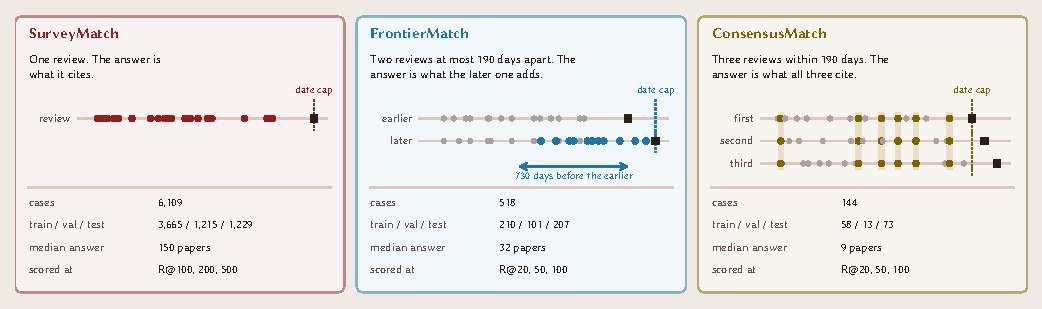
\includegraphics[width=\textwidth]{figures/benchmarks.pdf}
\Description{Three cards, one per benchmark, each with a timeline schematic and a table of counts. SurveyMatch: one review, whose references are all colored as the answer, with the date cap at the review; 6,109 cases split 3,665 train, 1,215 validation, 1,229 test; a median answer of 150 papers; scored at R@100, 200, and 500. FrontierMatch: two reviews at most 190 days apart, an earlier and a later one, where only the references the later one adds are colored, the date cap sits at the earlier review, and an arrow marks the 730 days before it; 518 cases split 210, 101, 207; a median answer of 32 papers; scored at R@20, 50, and 100. ConsensusMatch: three reviews within 190 days, where only the references all three share are colored and joined by vertical bands, with the date cap before the reviews; 144 cases split 58, 13, 73; a median answer of 9 papers; scored at R@20, 50, and 100.}
\caption{The proposed benchmarks. Each row is one review on a timeline with its references as dots, the answer in color, and the date cap the retriever is held to. The schematics are illustrative and the counts are from the 2026-10-22 release.}
\label{fig:benchmarks}
\end{figure*}

\subsubsection{Proposed Benchmarks}

Existing benchmarks fall short of real literature research in three ways: most pair a query with a few papers while a review cites over 100, their keys are chosen by annotators or LLMs rather than by researchers for their own work, and each case comes from a single source paper. We addressed all three by mining benchmarks from GraphIV's own reviews (\cref{fig:benchmarks}), whose reference lists are large keys written by researchers. The topic tree and the survey classifier also let us group several reviews of one topic into a case, which to our knowledge no existing benchmark does, to ask what a field added over time and what it agrees on.

A review is a paper with a survey probability of at least 0.95, where the classifier's precision is 0.937, and its references are the papers it cites that resolved in GraphIV and predate it. Gemma 4 26B wrote each case's research question from the titles, frozen in the release.

\begin{itemize}
    \item \textbf{SurveyMatch} asks what a review cites. A case is one review with at least 100 references, which are its answers.
    \item \textbf{FrontierMatch} asks what a field picked up over a short period. A case is two reviews in one topic leaf, at most 190 days apart with a cosine of at least 0.80, and its answers are what the later review cites and the earlier does not, dated at most 730 days before the earlier one.
    \item \textbf{ConsensusMatch} asks what every review of a topic agrees on. A case is three reviews in one leaf within 190 days, each pair at a cosine of at least 0.75, and its answers are what all three cite.
\end{itemize}

We split cases by hashing their anchors' arXiv ids, so a newer release is strictly additive. SurveyMatch is scored at R@100, 200, and 500, and the smaller FrontierMatch and ConsensusMatch at R@20, 50, and 100.

\subsection{Retrieval (BoundedField)}
\label{sec:bf}

BoundedField is an LLM-free, citation-aware retriever. Given a question, it retrieves the 5,000 papers most cosine-similar to it, dated on or before its cap. The top 200 form the \term{core}, and expanding the list by one citation hop to and from the core gives the \term{pool}.

\paragraph{Walking the citation graph:}
Let $A \in \{0,1\}^{|P| \times |P|}$ be the citation graph on the \term{pool} $P$, where $A_{ij} = 1$ if paper $j$ cites paper $i$, and $c\in\mathbb{R}^{|P|}$ the core's cosines, zero elsewhere, normalized to sum to one. Multiplying by $A$ walks one hop back in time and by $A^\top$ one hop forward, so graph traversal reduces to matrix products. Each walk gives a raw term $u_\tau \in \mathbb{R}_{\geq 0}^{|P|}$:
\begin{equation}
    \label{eq:walks}
    \begin{aligned}
        u_{\text{anc}} &= A c, & u_{\text{fro}} &= A^\top c, & u_{\text{cocite}} &= (A A^\top c) \odot r, \\
        u_{\text{anc2}} &= A^2 c, & u_{\text{fro2}} &= (A^\top)^2 c, & u_{\text{couple}} &= (A^\top A c) \odot r.
    \end{aligned}
\end{equation}
$Ac$ is what the core cites, $A^\top c$ what cites it, and $AA^\top c$ and $A^\top A c$ are co-citation \citep{small1973cocitation} and bibliographic coupling \citep{kessler1963coupling} seeded by the core, weighted by the recency $r_p = 1/(1+a_p)$ of a paper aged $a_p$ years at the cap. We write $W$ for these six walks.

\paragraph{Additional terms:}
BoundedField also scores the cosine $u_{\text{cos}}$, the recency $u_{\text{rec}} = r$, and the question's BM25 within the pool $u_{\text{bm25}}$ \citep{robertson2009bm25}. As $u_{\text{anc}}$ and $u_{\text{fro}}$ are zero beyond the core's direct neighbors, two decay terms $u_{\text{anc\_decay},p} = \delta^{d^{\leftarrow}(p)}$ and $u_{\text{fro\_decay},p} = \delta^{d^{\rightarrow}(p)}$, with $\delta = 0.5$, let farther papers score, where $d^{\leftarrow}(p)$ and $d^{\rightarrow}(p)$ are the fewest hops from the core walking $A$ and $A^\top$, up to 4, and the term is zero beyond. The hub term counts a paper's citations across all of GraphIV, $u_{\text{hub},p} = \sum_{j : t_j \leq t} \tilde{A}_{pj}$, for the full graph $\tilde{A}$, cap $t$, and paper dates $t_j$, excluding the case's anchors.

\paragraph{Bounding the terms:}
The raw terms are not comparable across queries: a walk grows with the size of the pool and the core, and its values are heavy-tailed, as a few landmark papers sit orders of magnitude above the rest. We therefore mapped every raw term $u_\tau$ to a bounded term $x_\tau \in [0,1]^{|P|}$, with a per-query normalization $N$ and, for the walks and hub, a compression $C_\lambda$:
\begin{gather*}
    N(v) = \frac{\max(v,0)}{\max_i \max(v_i,0)}, \\
    C_\lambda(v) = N\bigl(\log(1 + \lambda\,N(v))\bigr), \qquad \lambda = 100,
\end{gather*}
\begin{equation*}
    x_\tau =
    \begin{cases}
        C_\lambda(u_\tau) & \tau \in W \cup \{\text{hub}\}, \\
        u_\tau & \tau \in \{\text{anc\_decay}, \text{fro\_decay}\}, \\
        N(u_\tau) & \text{otherwise}.
    \end{cases}
\end{equation*}
$N$ is invariant to scale, $N(\alpha v) = N(v)$ for $\alpha > 0$, so a bounded term depends only on how the papers of one pool compare with each other. $C_\lambda$ preserves order and zeros and maps the top paper to 1, but lifts a paper at 1\% of the top from 0.01 to $\log 2 / \log 101 \approx 0.15$, so $\lambda$ sets how far below the top a term still separates papers. The decay terms already lie on $[0,1]$ and are left as they are. We then combined the bounded terms as a product of bounded factors:
\begin{equation}
    \label{eq:bf}
    \begin{aligned}
        \mathrm{score}(p) &= \frac{\prod_{\tau \in T} \left(1 + x_{\tau,p}\right)^{w_\tau}}{\left(1 + x_{\text{hub},p}\right)^{w_{\text{hub}}}}, \\
        \log \mathrm{score}(p) &= \sum_{\tau \in T} w_\tau \,\phi_{\tau,p} - w_{\text{hub}}\, \phi_{\text{hub},p},
    \end{aligned}
\end{equation}
where $T$ is every term but hub, $w_\tau \geq 0$, and $\phi_{\tau,p} = \log(1 + x_{\tau,p})$. This makes BoundedField fundamentally a linear ranking function over fixed, bounded features. A missing term is ignored (at 0 in the summation), meaning papers too new to be cited (with $x_{\text{anc}} = 0$) are not excluded. The exponents $w_\tau$ are what we tuned for each task (\cref{sec:tuning}).

\subsection{Automated Research System}
\label{sec:mcp}

GraphIV-MCP gives an LLM agent six tools over the Model Context Protocol \citep{anthropic2024mcp}, and the client owns the agent loop, turning the user's question into a sequence of calls. Our agent is an open-weight fine-tune of Qwen3.6 27B \citep{qwen2026qwen36}, served through llama.cpp \citep{gerganov2023llamacpp} on the same RTX 3090. The following tools are available:
\begin{itemize}
    \item \texttt{search\_papers} runs BoundedField with a specific recipe
    \item \texttt{recall\_paper} finds the one paper that best matches a description
    \item \texttt{read\_paper} answers a question about a paper in claims backed by verbatim quotes
    \item \texttt{list\_citations} returns a paper's citers or references with their intents and citing sentences
    \item \texttt{trace\_lineages} follows \term{extends}, \term{compares}, and \term{critiques} citations through a set of papers
    \item \texttt{save\_report} saves the report once every citation in it resolves to a quote the agent read
\end{itemize}
\Cref{app:agent} details each tool and the agent's effort presets, and \cref{app:questions} lists the 21 test questions.
